\chapter{Grundlagen solarthermischer Wärmebereitstellung}\label{section: Solarthermische Wärmebereitstellung}
\thispagestyle{empty}

In der Literatur zu regenerativen Energiesystemen wird die Wärmegewinnung durch Solarthermie ausschließlich für die häusliche Anwendung betrachtet (\citet{Quaschning2015} und \citet{Watter2013}). Obwohl sich diese Arbeit mit dem Einsatz in Wärmenetzen  beschäftigt, bleibt die Technologie unverändert. Aus diesem Grund wird auf eine Beschreibung der Funktionsweise solarthermischer Kollektoren verzichtet. Dieser Abschnitt stellt zunächst dar, wie gemessene Daten der Sonneneinstrahlung auf eine horizontale Ebene umgerechnet werden können, um die Einstrahlung auf eine geneigte Ebene abzubilden. Anschließend wird der Ansatz zur Bewertung solarthermischen Anlagen dargestellt. Schließen wird dieser Abschnitt in einer Besprechung möglicher Konzepte zur solarthermischen Wärmebereitstellung.

\section{Funktionsweise}\label{Funktionsweise Solarthermische Wärmebereitstellung}
Bei der Solarthermie wird das Licht der Sonne in Wärme umgewandelt. Grundlage für die Berechnung solarthermischer Anlagen ist das Stefan-Boltzmann-Gesetz (Gleichung \ref{equation: Stefan-Boltzmann-Gesetz}), welches die Wärmestrahlung $\dot{Q}$ eines Körpers beschreibt \cite{stefan1879}. Die thermischen Verluste eines Kollektors, aber auch die abgegebene Strahlung der Sonne lassen sich über dieses Gesetz berechnen. 
\begin{equation}\label{equation: Stefan-Boltzmann-Gesetz}
\dot{Q} = \varepsilon \cdot \sigma_\text{s} \cdot A \cdot T^4
\end{equation}
\begin{tabbing}
	\hspace{1cm}\=\hspace{0.5cm}\=\hspace{0.5cm}\=\hspace{1cm}\=\kill
	\> $\dot{Q}$ \>: \> Wärmestrahlung eines Körpers\\
	\> $\varepsilon$ \>:  \> Emissionsgrad des Körpers\\
	\> $\sigma_\text{s}$ \>: \> Stefan-Boltzmann-Konstante\\
	\> $A$ \>: \> Oberfläche des Körpers\\
	\> $T$ \>: \> Oberflächentemperatur des Körpers\\
\end{tabbing}
Außerhalb der Erdatmosphäre beträgt die Wärmestrahlung der Sonne im Durchschnitt noch $1360,8 \pm 0,5 \frac{\text{W}}{\text{m}^2}$ \cite{Quaschning2015}. Die Strahlung, welche schließlich die Erdoberfläche erreicht, fällt aufgrund der Atmosphäre geringer aus. Gemessen wird diese Globalstrahlung $E_\text{G,hor}$ bezogen auf die horizontale Ebene \cite{DWDstrahlung}. Sie setzt sich aus einem direkten Anteil $E_\text{dir,hor}$ und einem diffusen Teil $E_\text{diff,hor}$ zusammen - dargestellt in Gleichung \ref{equation: E_hor}. Sollte bei der Messung ausschließlich die Globalstrahlung angeben sein, kann diese über statistische Verteilungen auf den direkten und diffusen Anteil umgerechnet werden \cite{Quaschning2015}.
\begin{equation}
\label{equation: E_hor}
E_\text{G,hor} = E_\text{dir,hor} + E_\text{diff,hor}
\end{equation}
Die Einstrahlung auf die horizontale Ebene ist für geneigte Kollektoren unter Berücksichtigung des Sonnenverlaufs umzurechnen, um realistische Ergebnisse für den Ertrag der Kollektoren zu erhalten. Ein möglicher Ansatz ist der in der DIN 5034-2 \cite{DIN5034} vorgeschlagenen Algorithmus zur Berechnung der Sonnenhöhe $\gamma_\text{s}$ und des Sonnenazimut $\alpha_\text{s}$. Dieser kann in Anhang \ref{Anhang: Sonnenstand} nachgeschlagen werden.

Der direkte Strahlungsanteil auf den Kollektor $E_\text{dir,gen}$ kann nach Bestimmung der entsprechenden Winkel über die in Gleichung \ref{equation: Winkelbeziehung} beschriebene Beziehung erfolgen. In Abbildung \ref{fig: Sonneneinstrahlung auf geneigter und Horizontaler Ebene} werden alle benötigten Winkel bei der Berechnung anschaulich dargestellt. Hierin stellt $\Theta_\text{gen}$ den Einfallswinkel zwischen dem Normalenvektor der Ebene und Sonne dar - $\gamma_\text{s}$ den Winkel zwischen der horizontalen und dem Sonnenstand.
\begin{equation}\label{equation: Winkelbeziehung}
E_\text{dir,gen} = E_\text{dir,hor} \cdot \dfrac{\cos \Theta_\text{gen}}{\sin \gamma_\text{s}}
\end{equation}

\begin{figure}[ht]
	\centering
	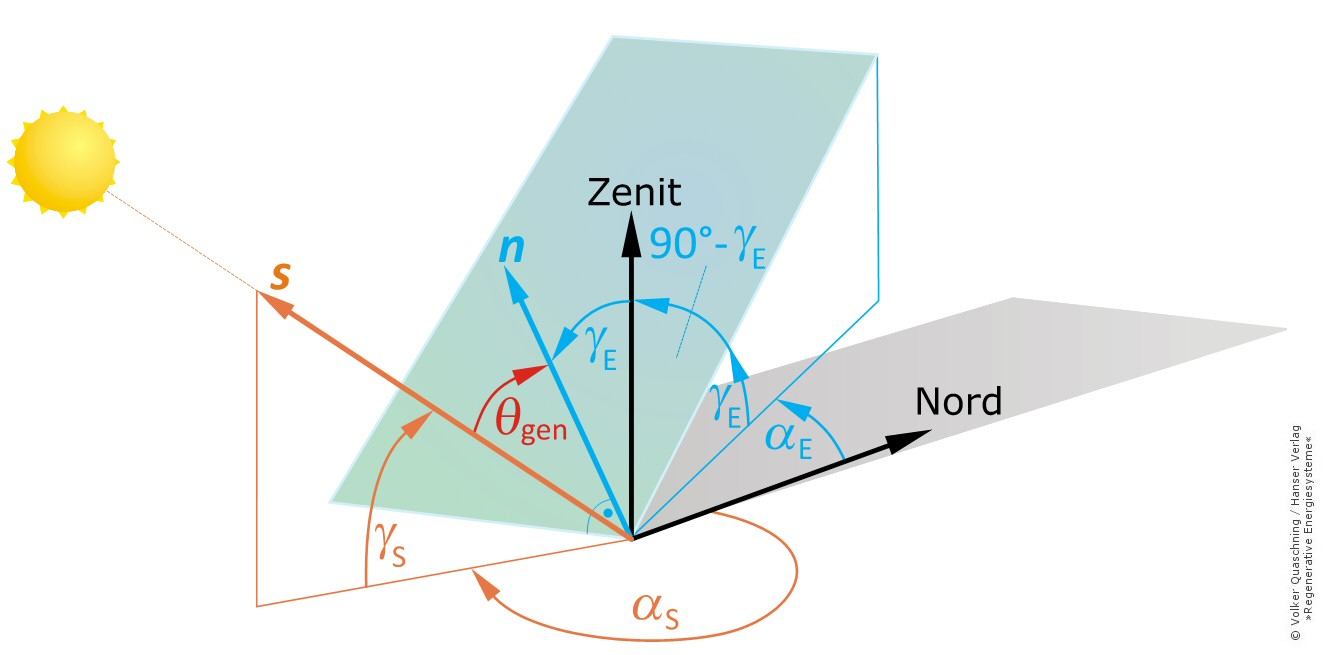
\includegraphics[width=0.8\linewidth]{Quaschning_Neigung.jpg}
	\captionof{figure}{Darstellung der Sonnenhöhe $\gamma_\text{s}$ und des Einfallswinkels $\Theta_\text{gen}$ zur Berechnung der Sonneneinstrahlung auf eine geneigte Ebene aus \citet{Quaschning2015}}
	\label{fig: Sonneneinstrahlung auf geneigter und Horizontaler Ebene}
\end{figure}
Zur Bestimmung der diffusen Einstrahlung auf die geneigte Ebene $E_\text{diff,gen}$ stehen verschiedene Ansätze zur Auswahl. In dieser Arbeit wird das Modell von \citet{KLUCHER1979} verwendet, da dieses nach \citet{Quaschning2015} eine relativ genaue Berechnung -~bei geringem Rechenaufwand~- liefert. In dem Modell von Klucher stellt der Faktor $F$ eine Hilfsgröße bei der Umrechnung dar und wird nach Gleichung \ref{equation: F} über die gemessene globale $E_\text{diff,hor}$ und diffuse Strahlung $E_\text{G,hor}$ auf die horizontale Ebene bestimmt. 
\begin{equation}
\label{equation: F}
F = 1 - \left( \dfrac{E_\text{diff,hor}}{E_\text{G,hor}} \right)^2 
\end{equation}
Dieser Faktor wird schließlich in Gleichung \ref{equation: E_diff_gen}, zusammen mit dem Aufstellwinkel der Ebene $\gamma_\text{e}$, dem Sonnenstandwinkel $\gamma_\text{s}$ und Einfallswinkel $\theta_\text{gen}$, genutzt, um die diffuse Einstrahlung auf die geneigte Ebene zu berechnen.
\begin{equation}\label{equation: E_diff_gen}
E_\text{diff,gen} = E_\text{diff,hor} \cdot \dfrac{1 + \cos \gamma_\text{s}}{2} \cdot \left( 1 + F \cdot \sin^3 \dfrac{\gamma_\text{e}}{2} \right) \cdot (1 + F \cos^2 \theta_\text{gen} \cdot \cos^3 \gamma_\text{s})
\end{equation}
Zusätzlich zur direkten und diffusen Einstrahlung auf die geneigte Ebene kommt ein kleiner Teil durch Bodenreflexion hinzu. Dieser hängt von dem Neigungswinkel $\gamma_\text{e}$ der Kollektoren und dem Albedo\footnote{Rückstrahlungsvermögen von nicht selbstleuchtenden, diffus reflektierenden Oberflächen}-Wert $A$ des Bodens ab. Die Berechnung des reflektierten Strahlungsanteils wird in Gleichung \ref{equation: E_refl_gen} dargestellt.
\begin{equation}
\label{equation: E_refl_gen}
E_\text{refl,gen} = E_\text{diff,hor} \dfrac{A (1 - \cos \gamma_\text{e})}{2}
\end{equation}
Schließlich ergibt sich die gesamte Einstrahlung  auf die geneigte Ebene nach Gleichung \ref{equation: E_G_gen} aus der Summe des direkten, diffusen und reflektierten Anteils. Abbildung \ref{fig: Vergleich horizontal vs geneigt} veranschaulicht den Gewinn, der durch die Neigung der Kollektorfläche erzielt wird.
\begin{equation}
\label{equation: E_G_gen}
E_\text{G,gen} = E_\text{dir,gen} + E_\text{diff,gen} + E_\text{refl,gen}
\end{equation}
Der gesamte DIN-Algorithmus zur Sonnenstandberechnung und Umrechnung der Einstrahlung auf die geneigte Ebene ist im Rahmen dieser Arbeit in ein Python-Skript geschrieben worden, welches dem beigefügten Datenträger entnommen werden kann.
\begin{figure}[ht]
	\centering
	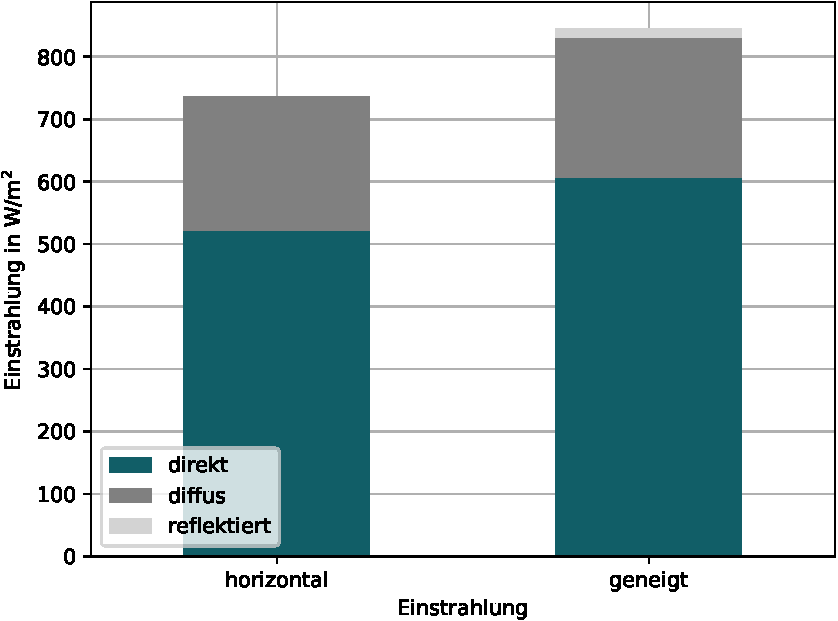
\includegraphics[width=0.8\linewidth]{radiation_on_horizontal_tilted.pdf}
	\captionof{figure}[Vergleich der Einstrahlung auf die horizontale und die geneigte Ebene]{Vergleich der Einstrahlung auf die horizontale und die geneigte Ebene. Die Rechnung ist beispielhaft für den 21.06.2016 um 14:00 Uhr, anhand der für diese Arbeit verwendeten Strahlungsdaten durchgeführt worden.}
	\label{fig: Vergleich horizontal vs geneigt}
\end{figure}

Die Effizienz $\eta_\text{K}$ der Kollektoren kann nun über den Quotienten der Nutzleistung $\dot{Q}_\text{N}$ und der  Einstrahlung auf den Kollektor mit der Fläche $A_\text{K}$ errechnet werden.
\begin{equation}\label{equation: exakter Kollektorwirkungsgrad}
\eta_\text{K} = \dfrac{\dot{Q}_\text{N}}{E_\text{G,gen} \cdot A_\text{K}}
\end{equation}	
Eine gute Annäherung für den Kollektorwirkungsgrad kann durch ein Polynom 2. Grades erreicht werden, wie es beispielsweise in DIN EN 12975 \cite{EN12975} vorgeschlagen ist. Der Wirkungsgrad wird, wie in Gleichung \ref{equation: EN12975} dargestellt, als Funktion der Temperaturdifferenz zwischen der mittleren Kollektortemperatur $T_\text{K}$ und Umgebungstemperatur $T_\text{U}$ angegeben. Dieses Verfahren wird beispielsweise von \citet{YANG2017471} zur Modellierung solarthermischer Anlagen bei einer Untersuchung zur Betriebsoptimierung in Wärmenetzen verwendet.
\begin{equation}\label{equation: EN12975}
\eta_\text{K} = \eta_\text{K,0} - \alpha_1 \cdot \dfrac{T_\text{K} - T_\text{U}}{E_\text{G,gen}} - \alpha_2 \cdot \dfrac{(T_\text{K} - T_\text{U})^2}{E_\text{G,gen}}
\end{equation}
\begin{equation}
T_\text{K} = \dfrac{T_\text{Eintritt} + T_\text{Austritt}}{2}
\end{equation}
Die Faktoren $\alpha_1$ [W/($m^2 K$)] und $\alpha_2$[W/($m^2 K^2$)] sind kollektorspezifisch und können dem Datenblatt des Herstellers entnommen werden. Der optische Wirkungsgrad $\eta_\text{K,0}$ gibt den maximal möglichen Wert an, der erreicht wird, wenn keine Temperaturdifferenz zwischen Fluid und Umgebung vorliegt. Tabelle \ref{tab: Kollektorparameter} gibt eine Übersicht über typische Werte für verschiedene Kollektorarten sowie ihre selektiven\footnote{Selektive Absorber verfügen über wellenlängenabhängige Transmissions-/Emissionskoeffizienten. Sie absorbieren Licht $< 2 \mu$m, welches den Hauptteil der Sonnenstrahlung ausmacht. Oberhalb von $2 \mu$m ist der Koeffizient möglichst gering, damit der Absorber nur wenig Wärme wieder an die Umgebung abgibt \cite{Quaschning2015}} und nicht selektiven Varianten.
\begin{center}
	\captionof{table}{Übersicht über typische Verlustkoeffizienten $\alpha_1$, $\alpha_2$ und $eta_\text{K,0}$ gängiger Kollektortypen aus \cite{Quaschning2015}}
	\begin{tabular}{llll}
		\hline 
		\rule{0pt}{12pt} Kollektortyp  & $eta_\text{K,0}$  & $\alpha_1$  & $\alpha_2$\tabularnewline
		\hline 
		
		Unverglaster Absorber  & 0,91  & 12  & 0  \tabularnewline
		Flachkollektor, Einfachverglasung, nicht selektiver Absorber & 0,86 & 6,1 & 0,025 \tabularnewline
		Flachkollektor, Einfachverglasung, selektiver Absorber  & 0,81 & 3,8 & 0,009 \tabularnewline
		Flachkollektor, Doppelverglasung, selektiver Absorber & 0,73 & 1,7 & 0,016 \tabularnewline
		Vakuumröhrenkollektor & 0,8 & 1,1 & 0,008 \tabularnewline
		\hline
		\label{tab: Kollektorparameter}  &  &  & 
	\end{tabular}
\end{center}
Das letzte Kriterium zur Bewertung solarthermischer Anlagen, welches im Rahmen dieser Arbeit Verwendung findet, ist der solare Deckungsgrad (\ac{SF}) nach Gleichung \ref{equation: SF}. Dieser gibt an, wie groß das Verhältnis aus solarthermisch gewonnener Wärme $Q_\text{ST}$ und des Wärmebedarfs $Q_\text{load}$ sowie der Wärmeverluste des Wärmenetzes $Q_\text{loss}$ ist \cite{YANG2017471}.
\begin{equation}
\label{equation: SF}
\text{\textit{SF}} = \dfrac{Q_\text{ST}}{Q_\text{load} + Q_\text{loss}}
\end{equation}

\section{Konzepte}\label{section: Konzepte}
Wie bei anderen Technologien auch, gibt es bei der Solarthermie verschiedene Möglichkeiten die Effizienz der Kollektoren oder des Gesamtsystems zu erhöhen. Die einfachste Methode stellt hier die Kombination mit anderen Wärmeversorgungstechnologien dar. \citet{ALBERGOSTERGAARD20104892} haben bereits dargelegt, dass Systeme, die einen großen Anteil regenerativer Energien aufweisen, aufgrund der volatilen Verfügbarkeit zur Versorgungssicherheit auf benachbarte Energiesysteme angewiesen sind. Entsprechend ist es bei isolierten Systemen notwendig, nicht regenerative Technologien als Back-Up zur Verfügung zu stellen. In dieser Arbeit wird ein bestehendes Versorgungssystem um drei unterschiedliche Solarthermie-Konzepte erweitert. Das bestehende System wird als Referenzsystem bezeichnet. 

Dieser Abschnitt gibt einen kurzen Überblick über verschiedene Ansätze zur Einbringung von Solarthermie in Wärmeversorgungsnetzen. Entsprechende Vor- und Nachteile der einzelnen Konzepte werden aufgeführt und eine begründete Auswahl für die drei zu untersuchenden Konzepte wird getroffen.

\subsection*{Alleinstehende Solarthermie}
Das einfachste Konzept und gleichzeitig mit den geringsten Investitionskosten ist die direkte Verwendung von solarthermischer Wärme in dem Wärmeversorgungssystem. Nachteilig bei diesem Konzept ist die Tatsache, dass Sonnenenergie zumeist dann zur Verfügung steht, wenn kein oder nur kaum Heizbedarf besteht. Eine Möglichkeit diesem Nachteil entgegen zu wirken ist die Verwendung von Wärmespeichern.

\subsection*{Solarthermie und saisonaler thermischer Energiespeicher}
	\begin{figure}[ht]
		\centering
		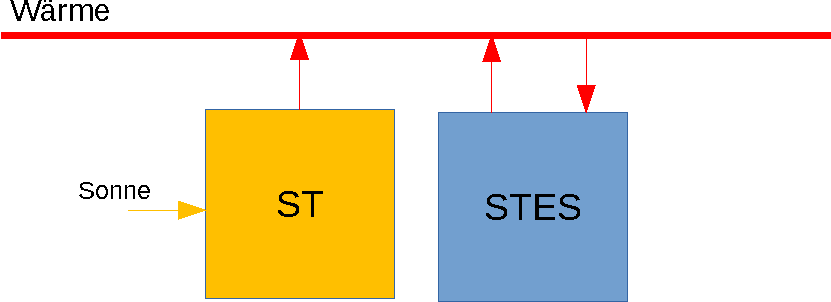
\includegraphics[width=0.8\linewidth]{ST+STES.pdf}
		\captionof{figure}[Schematische Darstellung eines Systems bestehend aus Solarthermie (ST) und einem saisonalen thermischen Energiespeichser (STES)]{Schematische Darstellung eines Systems bestehend aus einer Solarthermie-Anlage (ST), welche Sonneneinstrahlung in Wärme wandelt und an ein Wärmesystem abgibt. Ein saisonaler thermischer Energiespeicher (STES) kann zur Speicherung von Wärme genutzt werden.}
		\label{fig: ST+STES}
	\end{figure}
Dieses Konzept nutzt einen saisonalen thermischen Energiespeicher, um es zu ermöglichen, dass überschüssige solarthermische Wärme gespeichert und zu einem späteren Zeitpunkt im Wärmesystem genutzt werden kann. Abbildung \ref{fig: ST+STES} veranschaulicht dieses Konzept, welches im Folgenden auch als Basis-Solarthermie-Konzept bezeichnet wird.
Im Falle der saisonalen Speicherung entspricht dies typischerweise der Speicherung der Sonnenenergie über den Sommer und der Nutzung der gespeicherten Wärme im Winter, wenn kaum Sonnenstrahlung vorliegt und die Umgebungstemperaturen die Effizienz der Solarkollektoren soweit absenkt, dass diese nicht genutzt werden können.

\citet{CARPANETO2015714} haben bereits gezeigt, dass der Nutzen solarthermischer Anlagen durch den Einsatz von Wärmespeichern deutlich erhöht werden kann. In der Literaturrecherche zu dieser Arbeit konnte keine Quelle identifiziert werden, die Solarthermie ohne den Einsatz von Wärmespeichern untersucht. Aufgrund der Tatsache, dass es sich bei diesem Konzept um das einfachste in der Praxis verwendete Konzept handelt, ist dieses das erste, welches für eine weitere Detailuntersuchung ausgewählt wird. 

\subsection*{Solarthermie, \ac{STES} und zusätzliche Wärmequelle} 
	\begin{figure}[ht]
		\centering
		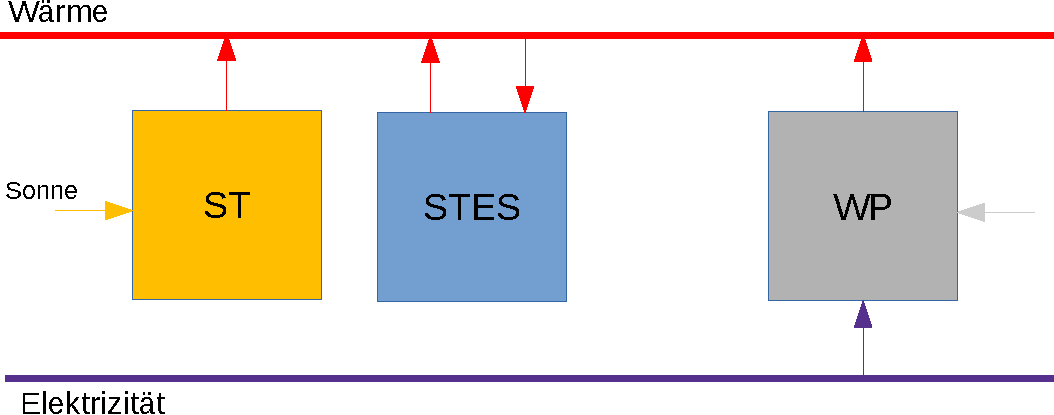
\includegraphics[width=0.8\linewidth]{ST+STES+HP1.pdf}
		\captionof{figure}[Schematische Darstellung eines um eine Kompressionswärmepumpe (WP) erweiterten Basis-Solarthermie-Konzepts]{Schematische Darstellung eines um eine Kompressionswärmepumpe (WP) erweiterten Basis-Solarthermie-Konzepts. Die Wärmepumpe nutzt Elektrizität um einen, nicht zu Heizzwecken nutzbaren Wärmestrom aufzuwerten und an das Wärmesystem abzugeben}
		\label{fig: ST+STES+HP1}
	\end{figure}
Bei diesem Konzept werden eine oder mehrere zusätzliche Wärmequellen parallel zu der Solarthermie verwendet. Diese können beispielsweise verschiedene Arten von Wärmepumpen, oder die Verbrennung von Biomasse sein. Generell lässt sich die Solarthermie mit allen möglichen Back-Up Wärmequellen kombinieren \cite{RAD20161550}. Im Rahmen dieser Arbeit wird jedoch ausschließlich die Kompressionswärmepumpe (WP) als zusätzliche Wärmequelle betrachtet, weil diese zusätzlich zur Sektorenkopplung zwischen Elektrizitäts- und Wärmeversorgung beiträgt. Außerdem weisen sie eine hohe Effizienz auf. Abbildung \ref{fig: ST+STES+HP1} zeigt das Basis-Solarthermie-Konzept, welches um eine \ac{WP} erweitert wurde, die Wärme aus der Umgebung oder Abwärme als Wärmequelle nutzt.

\subsection*{Solarthermie, \ac{STES}, \ac{WP} und \ac{STTES}}
Wärmepumpen haben den Vorteil, dass sie Phasen günstiger Strompreise nutzen können, um Wärme bereitzustellen. Diese fallen jedoch nicht unbedingt mit Bedarfsspitzen thermischer Energie zusammen. Durch die Einbringung eines Kurzzeitspeichers, der Wärme über mehrere Stunden speichern kann, ist es möglich die von der \ac{WP} bereitgestellte Wärme zeitlich von dem Bedarf zu entkoppeln. Abbildung \ref{fig: ST+STES+HP1+STTES} stellt das Konzept in einer entsprechend schematischen Darstellung vor.
	\begin{figure}[ht]
		\centering
		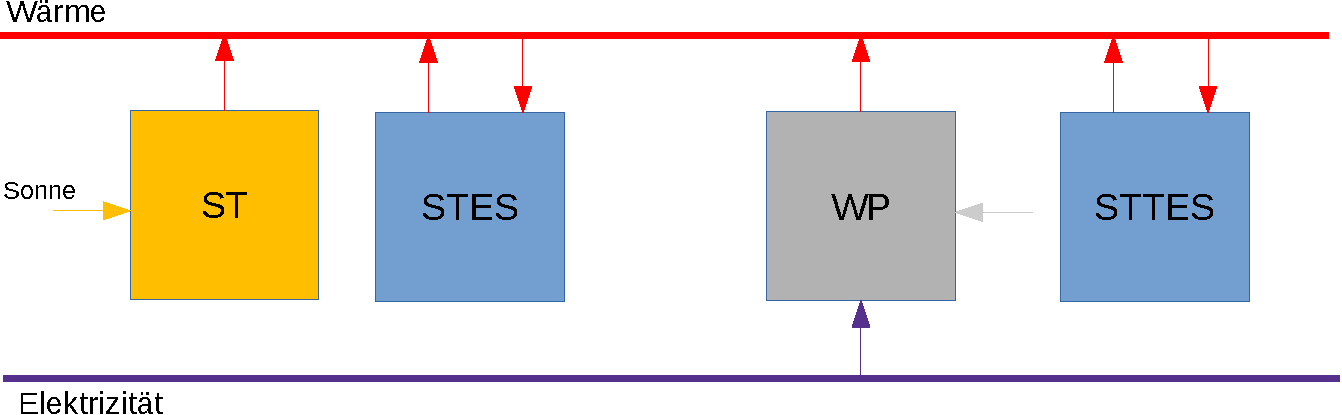
\includegraphics[width=0.8\linewidth]{ST+STES+HP1+STTES.pdf}
		\captionof{figure}[Schematische Darstellung eines Solarthermie-Konzepts mit Wärmepumpe und Kurzzeitspeicher]{Darstellung eines Basis-Solarthermie-Konzepts, welches um eine Wärmepumpe und einen Kurzzeitsspeicher erweitert worden ist. Der Kurzzeitspeicher entnimmt und beliefert das Wärmesystem mit Wärme und soll den Betrieb der Wärmepumpe optimieren}
		\label{fig: ST+STES+HP1+STTES}
	\end{figure}

Bei den zuletzt vorgestellten Konzepten sind die verwendeten Technologien ausschließlich parallel zu dem Basis-Solarthermie-Konzept geschaltet worden. Prinzipiell ein möglicher Nutzen, der durch die Verwendung einer Wärmepumpe und eines Kurzzeitspeichers erreicht wird, auch in einem Versorgungssystem ohne Solarthermie zu erwarten. 

Dieses Konzept ist für eine genauere Betrachtung im Rahmen dieser Arbeit ausgewählt worden, da durch den Einsatz einer Wärmepumpe und eines Kurzzeitspeicher das Wärmesystem einen erhöhten Anteil von \ac{P2H}-Technologien aufweist. Eine genauere Untersuchung wird zeigen, wie sich der Einsatz von Solarthermie auf ein System mit erhöhtem \ac{P2H}-Anteil auswirkt.  

\subsection*{Wärmepumpe zur Effizienzsteigerung der Solarthermiekollektoren}
Die vorangegangenen Konzepte haben ein bestehendes Solarthermie-System um weitere Technologien erweitert, die parallel zur Solaranlage geschaltet werden. Dies steigert die Effizienz des Gesamtsystems, hat jedoch keinen Einfluss auf die Effizienz der Solarthermie-Anlage. Wie aus Gleichung \ref{equation: EN12975} hervorgeht nimmt die Effizienz solarthermischer Anlagen mit abnehmender Kollektormitteltemperatur zu. Bei den bisher betrachteten Solarthermie Konzepten speist die Anlage direkt in das Wärmesystem ein. Daraus folgt, dass die Austrittstemperatur der Solaranlage mit der Vorlauftemperatur des Netzes übereinstimmt. Im Sommer liegt diese in typischen Fernwärmenetzen noch bei über 80\textdegree C \cite{stadtwerke_flensburg_gmbh_2019_2553968}. 
	\begin{figure}[ht]
		\centering
		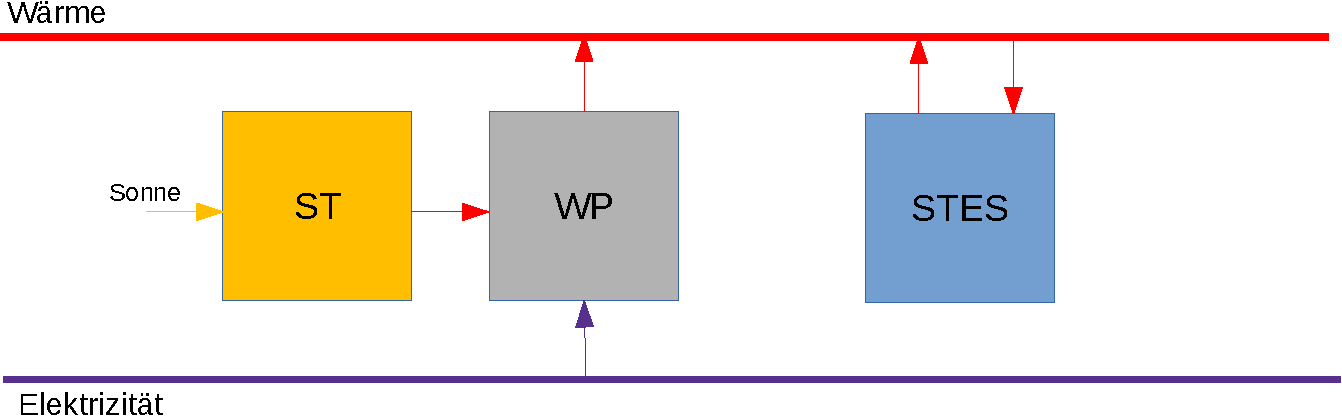
\includegraphics[width=0.8\linewidth]{ST+HP2.pdf}
		\captionof{figure}[Eine solarthermische Anlage liefert Wärme an eine Wärmepumpe zur Effizienzsteigerung]{Eine solarthermische Anlage speist in diesem Konzept nicht direkt ins Wärmesystem, sondern liefert zur Effizienzsteigerung Wärme bei einem niedrigeren Temperaturniveau an eine Wärmepumpe. Diese nutzt Elektrizität um das Temperaturniveau auf das Niveau des Wärmesystems anzuheben.}
		\label{fig: ST+HP2}
	\end{figure}

Bei diesem Konzept, welches in Abbildung \ref{fig: ST+HP2} dargestellt wird, können die Solarkollektoren auch bei geringeren Temperaturen als der Vorlauftemperatur betrieben werden, was zu einer Steigerung der Kollektoreffizienz und somit zu einem erhöhten Ertrag der Anlage führt. Außerdem kann die Wärmepumpe auch betrieben werden, wenn keine solarthermische Wärme bereitgestellt wird. Natürlich ist es ebenfalls möglich dieses Konzept  um zusätzliche Wärmequellen und Kurzzeitspeicher zu erweitern.

\subsection*{Steigerung der Speicherkapazität des \ac{STES} durch den Einsatz einer Wärmepumpe}	
Die minimale und maximale Temperatur eines Wärmespeichers ist von der Rücklauf- und maximalen Vorlauftemperatur des Wärmenetzes abhängig. Aus Gleichung \ref{equation: Speicherkapazität} geht bereits hervor, dass die Speicherkapazität direkt proportional zur Temperaturdifferenz $\Delta T$ ist. Durch den Einsatz einer Wärmepumpe kann die minimale Temperatur des Speichers unter die Rücklauftemperatur des Netzes gesenkt werden. Dieses Konzept wird in Abbildung \ref{subfigure: STES+HP3} dargestellt. 

Eine weitere Möglichkeit der Effizienzsteigerung ist die Einspeisung der solarthermischen Anlage in den Wärmespeicher anstatt direkt in das Wärmesystem einzuspeisen. Dieses Konzept, bei dem der Wärmespeicher generell bei einem geringeren Temperaturniveau betrieben wird, wurde von \citet{MARX2014} genauer betrachtet. Eine konzeptionelle Darstellung ist in Abbildung \ref{figure: ST+STES+HP3} dargestellt. Durch das reduzierte Temperaturniveau können die temperaturabhängigen Verluste verringert werden. Außerdem erhöht sich, wie im vorangegangen Konzept, die Effizienz der Solarthermie-Kollektoren. 
	\begin{figure}
		\begin{subfigure}[b]{0.48\textwidth}
			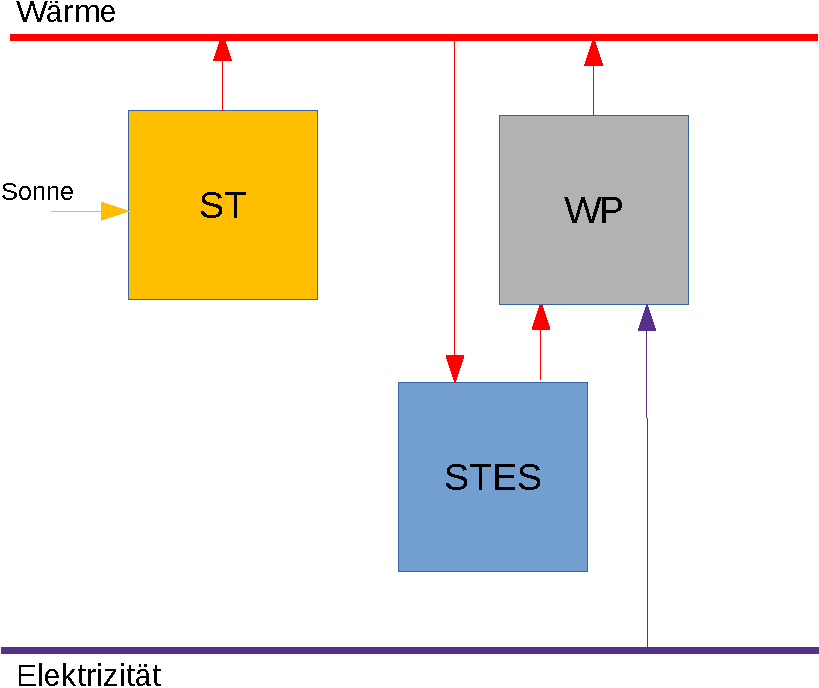
\includegraphics[width=1\textwidth]{STES+HP3.pdf}
			\subcaption{}
			\label{subfigure: STES+HP3}
		\end{subfigure}
		\hfill
		\begin{subfigure}[b]{0.48\textwidth}
			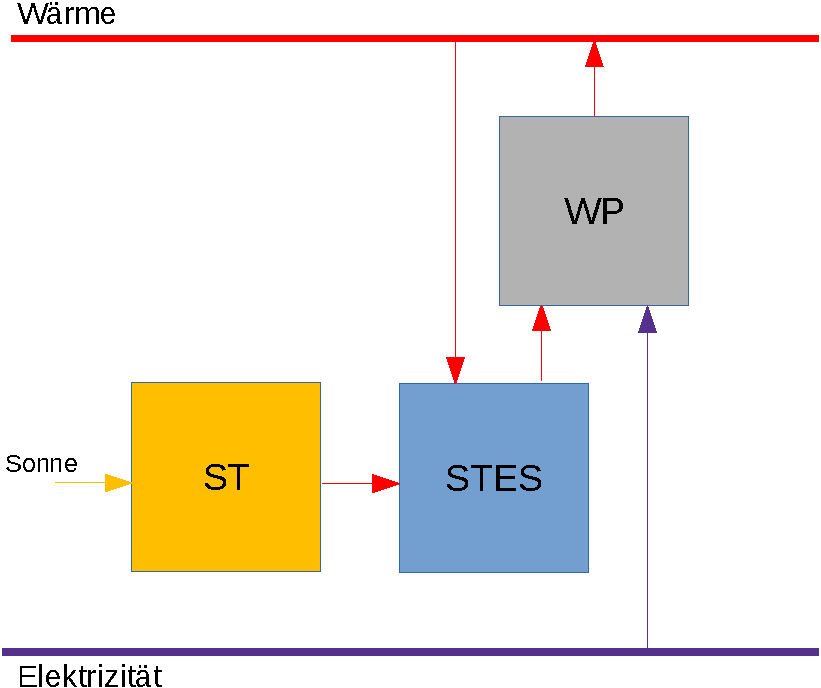
\includegraphics[width=1\textwidth]{ST+STES+HP3.pdf}
			\subcaption{}
			\label{figure: ST+STES+HP3}
		\end{subfigure}
		\caption[Konzeptionelle Darstellung zweier Ansätze zur Steigerung der Speicherkapazität durch Verwendung einer Wärmepumpe]{Konzeptionelle Darstellung zweier Ansätze zur Steigerung der Speicherkapazität durch Verwendung einer Wärmepumpe. In (a) wird eine Wärmepumpe genutzt, um einen \ac{STES} zu entladen, während eine Solarthermie-Anlage direkt ins Wärmesystem einspeist. In (b) speist die solarthermische Anlage direkt in den Speicher, der wiederum von einer Wärmepume entladen werden kann.}
		\label{fig: STES+HP}
	\end{figure}

\subsection*{Photovoltaik und Wärmepumpe}\label{subsection: Konzepte - Photovoltaik und Wärmepumpe}
	\begin{figure}[ht]
		\centering
		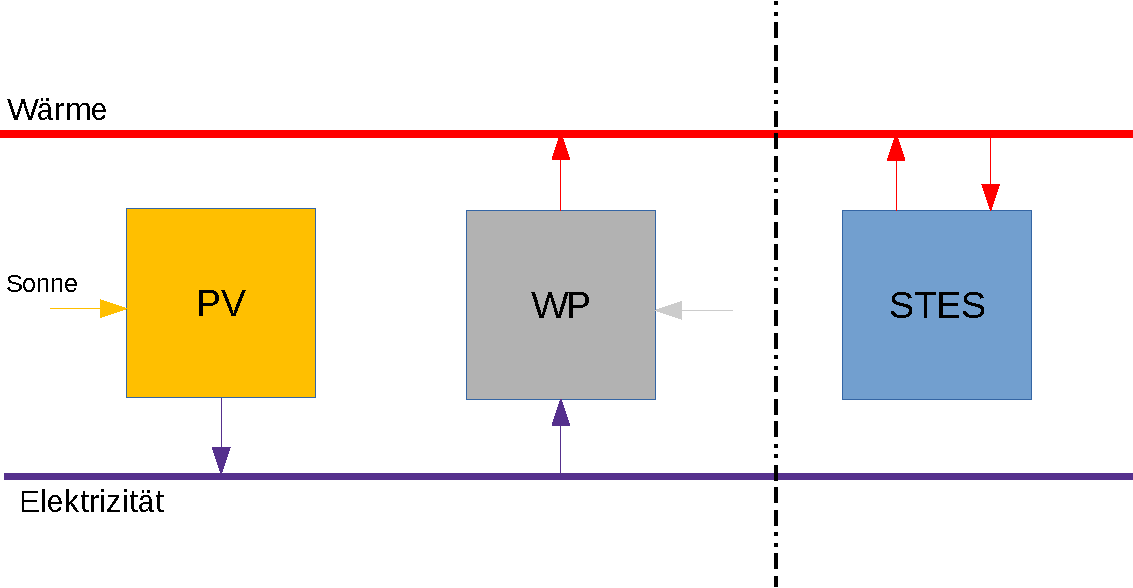
\includegraphics[width=0.8\linewidth]{Photovoltaik.pdf}
		\captionof{figure}[Schematische Darstellung eines Photovoltaik basierten Konzepts zur Wärmebereitstellung]{Schematische Darstellung eines Photovoltaik basierten Konzepts zur Wärmebereitstellung. Eine \ac{PV}-Anlage wandelt Sonneneinstrahlung in Elektrizität um, die wiederum von der Wärmepumpe genutzt werden kann, um Wärme bereitzustellen.}
		\label{Abbildung: PV-Konzept}
	\end{figure}
\citet{GRAVELSINS2019} haben ein Konzept vorgestellt, welches eine Alternative zur klassischen Solarthermie darstellt, in dem die Sonnenstrahlung indirekt genutzt wird, um Wärme bereitzustellen. Der durch die \ac{PV}-Anlage gewonnene Strom wird genutzt, um eine Wärmepumpe zu betreiben, die wiederum dem Wärmenetz Wärme bereitstellt. Dieses Konzept der \textit{indirekten} Solarthermie, welches in Abbildung \ref{Abbildung: PV-Konzept} dargestellt wird, bietet einige Vorteile gegenüber der klassischen Solarthermie. Zunächst haben \ac{PV}-Module den Vorteil, dass sie schwankenden Umgebungsbedingungen gegenüber unempfindlicher sind als Solarthermieanlagen. Eine sinkende Umgebungstemperatur hat beispielsweise, im Gegensatz zur Solarthermie, einen positiven Einfluss auf den Modul-Wirkungsgrad \cite{Quaschning2015}. Ein weiterer Vorteil ist, dass  die erforderliche Wärmepumpe einerseits unabhängig von der dargebotenen Strahlung eingesetzt und andererseits der \ac{PV}-Strom - je nach Preislage und Wärmenachfrage - direkt vermarktet werden kann.  

Ein weiterer Vorteil des \ac{PV}-Konzepts ist, dass die Investitionskosten von \ac{PV}-Modulen pro m² derzeit deutlich geringer ausfallen als bei Flach- oder Vakuumröhrenkollektoren. Darüber hinaus haben \citet{Vartiainen2019} dargelegt, dass in den nächsten Jahren weiter mit stark fallenden Preisen für die Photovoltaik zu rechnen ist. Tabelle \ref{tab: Preisvergleich PV/Solar} stellt die aktuellen Investitionskosten der verschiedenen Technologien von Anlagen jenseits der 100.000m² - die in Dänemark bereits eingesetzt werden - vergleichend gegenüber. Die Kosten für \ac{PV} sind \textit{Aktuelle Fakten zur Photovoltaik} \cite{ISE} entnommen worden, die Kosten der Solarthermie sind nach Gleichung \ref{equation: Kosten-Flachkollektor} und \ref{equation: Kosten-Vakuumkollektor} bestimmt worden. Aufgrund der zu erwartenden, anhaltenden Kostenreduktion von \ac{PV}-Modulen und der vielfältigen Möglichkeiten die Sonnenstrahlung zu nutzen ist dieses Konzept als drittes für eine weitere Detailanalyse ausgewählt worden.
\newpage
	\begin{center}
		\captionof{table}{Gegenüberstellung der spezifischen Investitionskosten zwischen Photovoltaik und Solarthermie für Anlagen > 100.000m²}
		\begin{threeparttable}
		\begin{tabular}{lcccl}
			\hline 
			\rule{0pt}{12pt} Technologie  & Einheit & Preis & Quelle & rel. Preis\tabularnewline
			\hline
			Photovoltaik (monokristallin)  &  \euro / kW$_\text{p}$ &  600 - 800 & \cite{ISE} & 1  \tabularnewline
			 & \euro/m² & $\approx$ 120 & & 1 \tabularnewline
			Flachkollektor & \euro/m²  & 190 & \cite{Waermenetz40}\tnote{1} & 1,6\tabularnewline
			Vakuumröhrenkollektor & \euro/m² & 245 & \cite{Waermenetz40} & 2,1\tabularnewline
			\hline
		\end{tabular}
		\begin{tablenotes}\footnotesize 
			\item[1] Grundlage für die Preisberechnung bildet \citet{Waermenetz40} (vgl. Gleichung \ref{equation: Kosten-Flachkollektor} und \ref{equation: Kosten-Vakuumkollektor}).
		\end{tablenotes}
	\end{threeparttable}
		\label{tab: Preisvergleich PV/Solar}
	\end{center} 
Folgende drei Konzepte werden im Rahmen dieser Arbeit weiter untersucht:
	\begin{description}
		\item[Solarthermie 1] Solarthermie und ein saisonaler thermischer Energiespeicher ergänzen das bestehende Referenzsystem. Diese Variante stellt das einfachste, aber zugleich das grundlegende solarthermische Konzept dar und ist aus diesem Grund als erstes Konzept für eine Detailuntersuchung ausgewählt worden.

		\item[Solarthermie 2] Hier wird das Solarthermie 1 Konzept zusätzlich um eine Wärmepumpe und einen Kurzzeitspeicher erweitert. Es ist ausgewählt worden, um den Einfluss der Solarthermie auf ein Wärmesystem mit erhöhtem \ac{P2H}-Anteil zu untersuchen.
		
		\item[Photovoltaik] Dieses Konzept stellt eine alternative Möglichkeit der solarthermischen Wärmebereitstellung dar. Die Solarthermie-Kollektoren sind durch eine Kombination aus \ac{PV}-Modulen und Wärmepumpen ersetzt worden. Dieses Konzept wurde ausgewählt, um zwei grundlegend verschiedene Konzepte zur Wärmebereitstellung aus Sonnenenergie miteinander zu vergleichen.		
	\end{description}